\documentclass[12pt, letterpaper] {article}

\parindent=5mm
\usepackage[spanish]{babel}

\usepackage{amssymb}
\usepackage{amsmath} 
\usepackage{amsfonts}

\usepackage[numbers,sort&compress]{natbib}
\usepackage{graphicx}

\usepackage{url}
\usepackage{hyperref}

\usepackage[top=25mm, bottom=20mm, left=1.5cm, right=1.5cm]{geometry}
\setlength{\parskip}{2mm}
\setlength{\parindent}{1pt}

\usepackage{listings}

\usepackage{float}

\usepackage[utf8]{inputenc}
\usepackage{graphicx} 
\usepackage{subfigure} 

\usepackage{color}
\usepackage{multirow}

\definecolor{dkgreen}{rgb}{0,0.6,0}
\definecolor{gray}{rgb}{0.5,0.5,0.5}
\definecolor{mauve}{rgb}{0.58,0,0.82}

\usepackage{color}
\usepackage{listings}
\lstset{ %
  language=R,                     % the language of the code
  basicstyle=\footnotesize,       % the size of the fonts that are used for the code
  numbers=left,                   % where to put the line-numbers
  numberstyle=\tiny\color{gray},  % the style that is used for the line-numbers
  stepnumber=1,                   % the step between two line-numbers. If it's 1, each line
                                  % will be numbered
  numbersep=5pt,                  % how far the line-numbers are from the code
  backgroundcolor=\color{white},  % choose the background color. You must add \usepackage{color}
  showspaces=false,               % show spaces adding particular underscores
  showstringspaces=false,         % underline spaces within strings
  showtabs=false,                 % show tabs within strings adding particular underscores
  frame=single,                   % adds a frame around the code
  rulecolor=\color{black},        % if not set, the frame-color may be changed on line-breaks within not-black text (e.g. commens (green here))
  tabsize=2,                      % sets default tabsize to 2 spaces
  captionpos=b,                   % sets the caption-position to bottom
  breaklines=true,                % sets automatic line breaking
  breakatwhitespace=false,        % sets if automatic breaks should only happen at whitespace
  title=\lstname,                 % show the filename of files included with \lstinputlisting;
                                  % also try caption instead of title
  keywordstyle=\color{blue},      % keyword style
  commentstyle=\color{dkgreen},   % comment style
  stringstyle=\color{mauve},      % string literal style
  escapeinside={\%*}{*)},         % if you want to add a comment within your code
  morekeywords={*,...}            % if you want to add more keywords to the set
} 


\author{Ricardo Rosas Macías}

\title{Práctica 10: algoritmo genético}

\date{\today}

\begin{document}

\maketitle


\section{Introducción}
En la práctica se aborda el problema de la mochila; mejor conocido como Knaspack, en el cual se busca la optimización de la combinación posible para la mezcla de artículos máximo que puede estar dentro de esta, en función al peso de cada uno. 

 \section{Objetivo}
Se realizó cambios en el c\'odigo proporcionado en la p\'agina web \cite{elisawebAG10}, de tal forma que la programación dinámica con ayuda de los algoritmos permite crear de una manera más sencilla la mejor combinación posible.
 
 \subsection{Descripción}
 
La finalidad del experimento es \cite{elisawebAG10}:
\begin{quotation}
 ``Paralelizar el algoritmo genético y estudia los efectos en su tiempo de ejecución con pruebas estadísticas y visualizaciones, variando el número de objetos en la instancia. Genere instancias con tres distintas reglas:
el peso y el valor de cada objeto se generan independientemente con una distribución normal,
el peso de cada objeto se generan independientemente con una distribución normal y su valor es correlacionado con el peso, con un ruido normalmente distribuido de baja magnitud, el peso de cada objeto se generan independientemente con una distribución normal y su valor es inversamente correlacionado con el peso, con un ruido normalmente distribuido de baja magnitud.\\
Asimismo, determinar para cada uno de los tres casos a partir de qué tamaño de instancia el algoritmo genético es mejor que el algoritmo exacto en términos de valor total obtenido por segundo de ejecución.''
\end{quotation}

\section{Resultados y conclusiones}

Se realizó el código en base a los antecedentes anteriormente reportados \cite{PGAM}. En las primeras líneas del c\'odigo se defini\'o los par\'ametros de experimentaci\'on con las cuales se trabajó; se estableció una serie de instancias como se describen en el objetivo. El código permite exhibir la eficiencia de selección de muestra en el experimento; siendo repetido 5 veces para obtener un valor estadístico más exacto. Además se paralelizó y configuró para que proporcione el tiempo que toma en ejecutar el código, de manera que logre mostrar las diferencias en tiempos de ejecución normal y paralelizada. 

\begin{lstlisting}[language=R]
startP=Sys.time()
n <- 50      
generaciones <- c(200, 250, 300)   
pmutaciones <- c(0.05, 0.1, 0.2)    
reproducciones <- c(50, 75, 100)   
iteraciones <- c(10, 15, 20)   
replicas <- 5 

datos <- data.frame(Replica = integer(), Optimo = integer(),
                    Generaciones = numeric(), ProbMut = numeric(),
                    Reproducciones = numeric(), Iteraciones = numeric(),
                    Objetivo = double())
cluster <- makeCluster(detectCores())
opt <- knapsack(capacidad, pesos, valores)[2]
clusterExport(cluster, "n")
clusterExport(cluster, "pesos")
clusterExport(cluster, "valores")
clusterExport(cluster, "capacidad")

for (tmax in iteraciones) {
  for (rep in reproducciones) {
    for (pm in pmutaciones) {
      for (init in generaciones) {
        for (r in 1:replicas) {
          
          #Inicio del genetico parsapply
          pobl <- t(parSapply(cluster, 1:init, function(i) {
            return(round(runif(n)))
          }))
          
          p <- as.data.frame(pobl)
          tam <- dim(p)[1]

            clusterExport(cluster, "p")
            clusterExport(cluster, "tam")
            
            probabilidades <- runif(tam) < pm
            mutados <- which(probabilidades %in% TRUE)
            
            mutaciones <- t(parSapply(cluster, mutados, function(i) {
              pos <- sample(1:n, 1)
              mut <- p[i,]
              mut[pos] <- (!p[i,][pos]) * 1
              return(as.numeric(mut))
            }))
            
            hijos <- matrix(parSapply(cluster, 1:rep, function(i) {
              padres <- sample(1:tam, 2, replace = FALSE)
              pos <- sample(2:(n-1), 1)
              x <- p[padres[1],]
              y <- p[padres[2],]
              xy <- c(x[1:pos], y[(pos+1):n])
              yx <- c(y[1:pos], x[(pos+1):n])
              return(as.numeric(c(xy, yx)))
            }), ncol = n, byrow = TRUE)
            
            p <- rbind(p, mutaciones, hijos)
            tam <- dim(p)[1]
            
            clusterExport(cluster, "p")
            clusterExport(cluster, "tam")
            
            p$obj <- parSapply(cluster, 1:tam, function(i) {
              return(sum(p[i,] * valores))
            })
            
            p$fact <- parSapply(cluster, 1:tam, function(i) {
              return(sum(p[i,] * pesos) <= capacidad)
            })
            
            mantener <- order(-p[, (n + 2)], -p[, (n + 1)])[1:init]
            
            p <- p[mantener,]
            tam <- dim(p)[1]
            
            assert(tam == init)
            
            factibles <- p[p$fact == TRUE,]
            mejor <- max(factibles$obj)
            mejores <- c(mejores, mejor)
            
          }
          
          datos <- rbind(datos, data.frame(Replica = r, Optimo = optimo,
                                           Generaciones = init, ProbMut = pm,
                                           Reproducciones = rep, Iteraciones = tmax,
                                           Objetivo = max(mejores)))
        }
      }
    }
  }
}
stopCluster(cluster)
endP=Sys.time()
\end{lstlisting}

En la figura \ref{NormPar} se puede observar en como la paralelización del experimento puede permitir minimizar los tiempos de ejecución. Asimismo, al incrementar la instancia se puede ver un comportamiento más abrupto en la ejecución normal, en comparación del paralelizado; que muestra ligeros cambios.

\begin{figure}[H]
\centering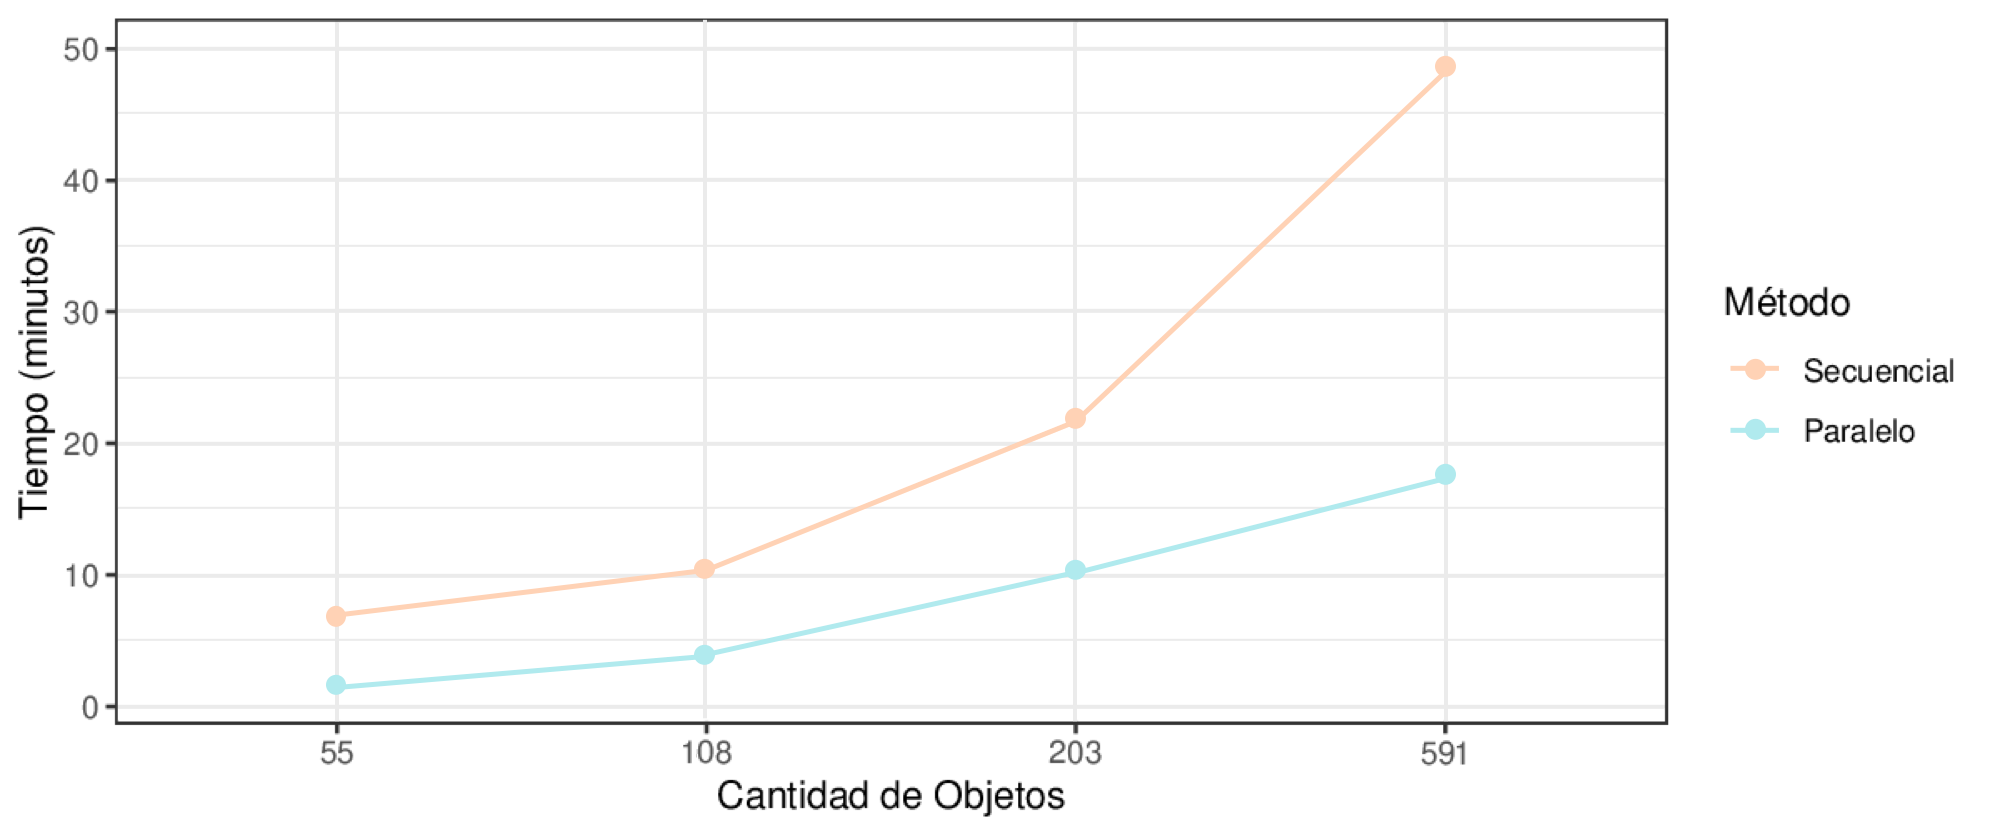
\includegraphics[width=170mm]{NormalParalelo.png}
\caption{Comparación de ejecución de código}
\label{NormPar}
\end{figure}

Con ayuda de la paquetería \textit{ggplot2} \cite{gg2} se obtuvo la visualización del error de la instancia creada, de modo que permite demostrar de manera cuantitativa el ruido del experimento. En la figura \ref{Perror} se logra denotar que al incrementar las variables este tiene un ruido que se mantiene constante en comparación con el comportamiento de las otras cantidades de generaciones. 

\begin{figure}[H]
\centering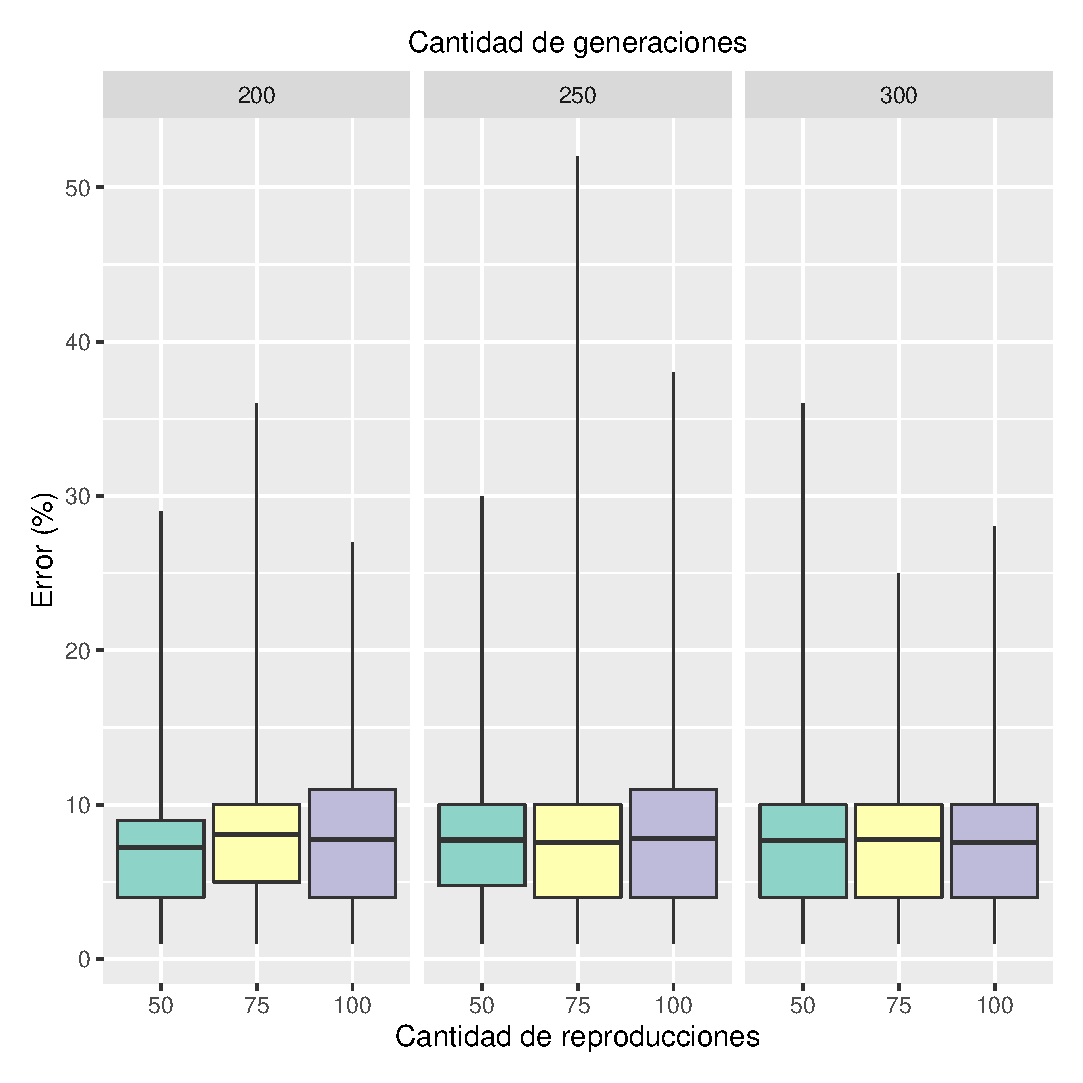
\includegraphics[width=98mm]{PError.eps}
\caption{Porcentaje de error respecto a las instancias generadas}
\label{Perror}
\end{figure}


\bibliographystyle{plainnat}

\bibliography{BiblioHWP10}

\end{document}